%% dvips -t letter -t landscape -I c philasug-111201
%% ps2pdf philasug-111201.ps philasug-111201.pdf

\documentstyle[slides-rmh,graphicx]{article}
\raggedbottom  %% overrides svsing7.sty default of \flushbottom

\textwidth 9.5in
\textheight 7in
\oddsidemargin  -.25in
\evensidemargin -.25in
\topmargin -1in
\setlength{\parindent}{0in}

\newcommand*{\Fortran}{\textsc{Fortran}}
\newcommand{\SAS}{{\textsc{SAS}}}
\def\url#1{\texttt{#1}} % To help fit in lines

\begin{document}
\thispagestyle{empty}
\Huge
\begin{center}
ESS (Emacs Speaks Statistics) as a User Interface to SAS
\vspace*{2ex}

Richard M. Heiberger\\
Temple University
\vspace*{2ex}
\end{center}


\begin{enumerate}
\item
Emacs is a mature, powerful, and easily extensible text editing system
that runs identically on all current computers (Unix, Windows, Macintosh, VMS).

Emacs knows the syntax of each programming language (Figure \ref{Image3}).

\begin{itemize}
\item directory editor
\item \Fortran
\item C
\item \LaTeX
\item \SAS
\item \SAS\ log
\item {\tt *Buffer List*}
\end{itemize}



\begin{figure}[tbp]
\vspace*{-.25in}
\hspace*{1.25in}
  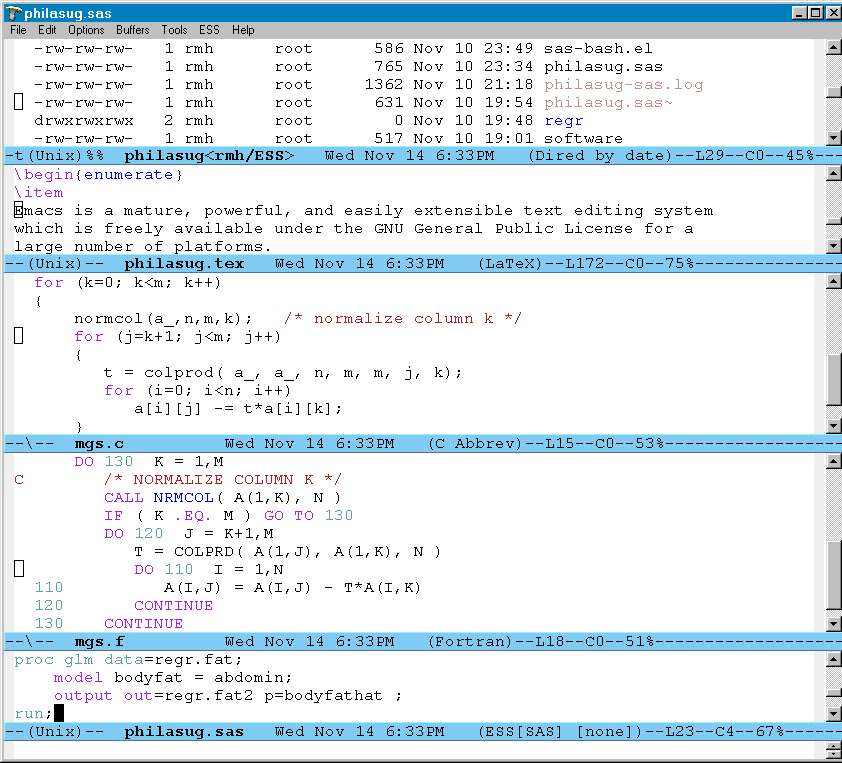
\includegraphics[angle=0,width=7.5in,natwidth=842,natheight=763]{Image3.png}
\vspace*{-.2in}
  \caption{Emacs frame with buffers showing a file directory,
\LaTeX\ file, C file, {\sc Fortran} file, and \SAS\ file.
Each file is syntactically highlighted for its language.}
  \label{Image3}
\end{figure}



\newpage
\item
Emacs can interact with and control other
programs either as subprocesses or as cooperating processes.
\setlength{\topsep}{1ex}
\begin{itemize}
\setlength{\itemsep}{1ex}
\item shell (Unix shell, on Unix or Windows machines)
\item msdos (on Windows machines)
\item telnet
\item SAS
\end{itemize}

One major advantage of running other processes under emacs is that the user
has complete search and editing capability on the interactive session.  The
interactive session is just another file that the computer is writing
to at the same time you are reading it.


\begin{figure}[tbp]
\vspace*{-.25in}
\hspace*{1.25in}
  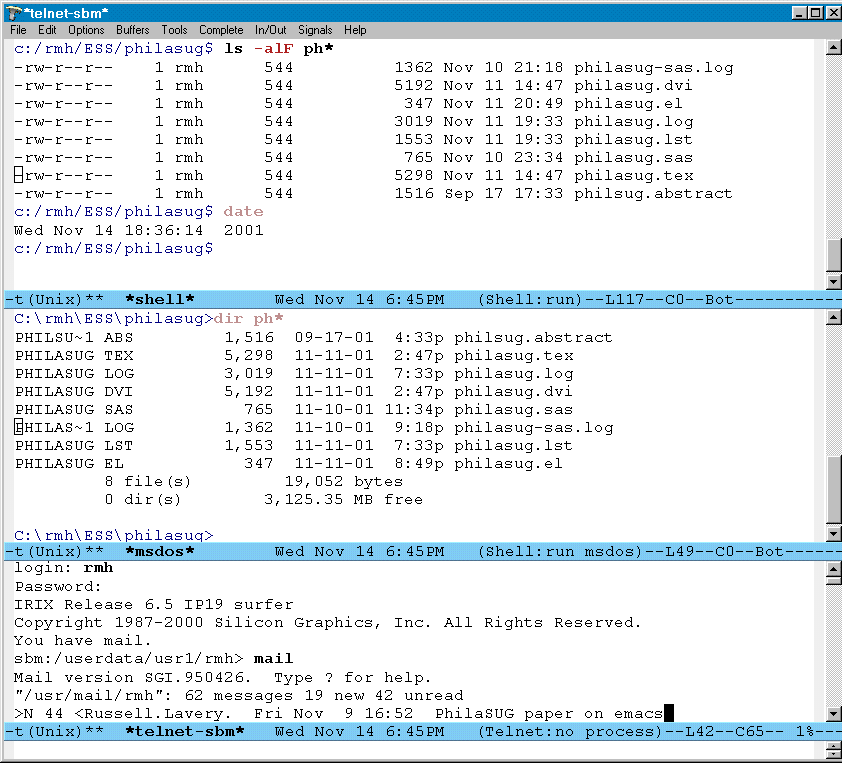
\includegraphics[angle=0,width=7.5in,natwidth=842,natheight=763]{Image4.png}
\vspace*{-.2in}
  \caption{Emacs frame with buffers showing a Cygwin Unix-like shell,
an MS-DOS shell, and a telnet session to a remote Unix computer.}
  \label{Image4}
\end{figure}

\newpage
\item
ESS extends Emacs to provide a functional and uniform\\
interface for
multiple statistical languages including SAS.\\[1ex]
%
The other languages ESS works with are
\setlength{\topsep}{1ex}
\begin{itemize}
\setlength{\itemsep}{1ex}
\item S (S-Plus and R)
\item XLispStat (including ARC and ViSta)
\item Stata
\end{itemize}
%
The programs can be running simultaneously on the same or different
computers.
\end{enumerate}
\newpage

Emacs provides:
\begin{itemize}
\setlength{\itemsep}{1ex}
\item viewing two or more files at once
\item editing formatted text
\item visual comparison of two similar files
\item syntax highlighting
\item syntactically appropriate indentation of text
\item enforcement of programming standards
\item navigation in units of
characters, words, lines, sentences, paragraphs, and pages.
\item all Unix utilities (grep, awk, etc, are builtin).
\end{itemize}


\begin{figure}[tbp]
  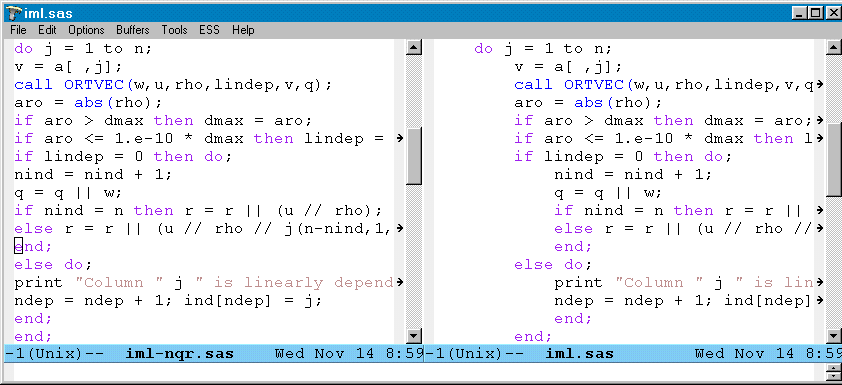
\includegraphics[angle=0,width=9.5in,natwidth=842,natheight=385]{Image5.png}
  \caption[]{Syntactically appropriate indentation of text.\\
Left: \SAS\ file as entered with all lines on the left margin.\\
Right: Same \SAS\ file indented by ESS to display nesting structure of statements.}
  \label{Image5}
\end{figure}

\begin{figure}[tbp]
  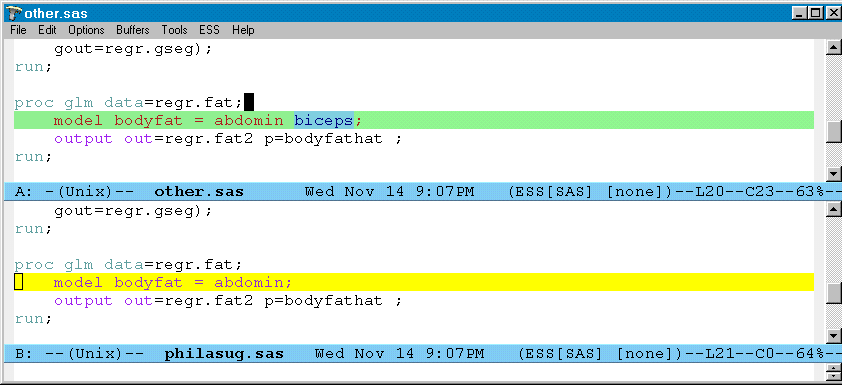
\includegraphics[angle=0,width=9.4in,natwidth=842,natheight=385]{Image7.png}
%  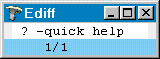
\includegraphics[angle=0,width=1.786in,natwidth=160,natheight=59]{Image6.png}
  \caption[]{Ediff session comparing two similar files.\\
The lines that differ are marked.\\
The words that differ on those lines are marked.}
  \label{Image7}
\end{figure}

\begin{figure}[tbp]
  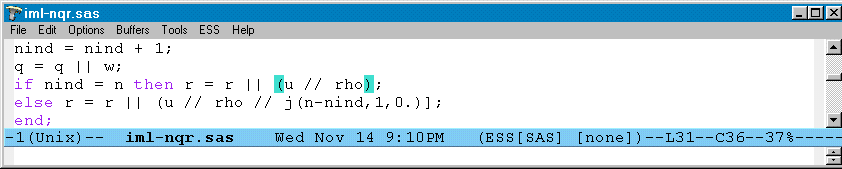
\includegraphics[angle=0,width=9.4in,natwidth=842,natheight=169]{Image8.png}

\vspace*{.5in}
  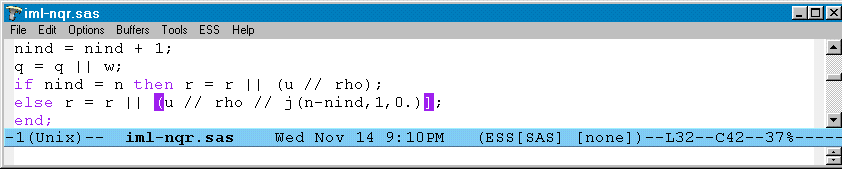
\includegraphics[angle=0,width=9.4in,natwidth=842,natheight=169]{Image9.png}
  \caption[]{Programming made easier.\\
Matching parentheses are highlighted in a gentle color.\\
Mismatching parentheses are highlighted in a disturbing color.\\
Keywords are in the keyword color.}
  \label{Image8-9}
\end{figure}


\begin{figure}[tbp]
  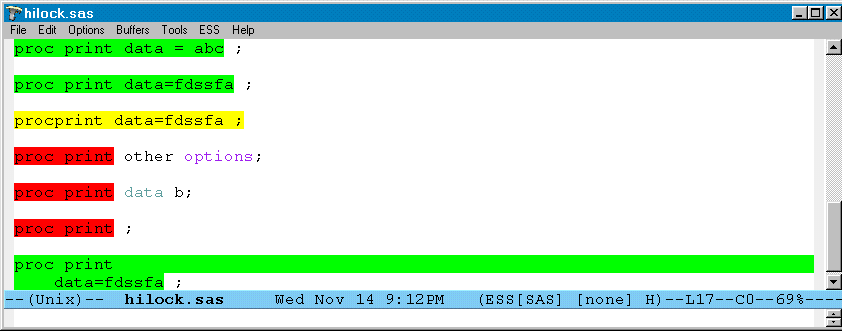
\includegraphics[angle=0,width=9.4in,natwidth=842,natheight=331]{Image10.png}
  \caption[]{Enforcement of programming standards.\\
  The standard says all {\tt PROC} statements
must have a {\tt DATA=datasetname} option.\\
Lines that satisfy the standard are green.\\
Lines that don't are red.\\
Lines that are unclear are yellow.}
  \label{Image10}
\end{figure}

\newpage
Learning emacs
\begin{itemize}
\setlength{\itemsep}{1ex}
\item TUTORIAL {\tt C-h t}
\item online manual {\tt C-h i}
\item reference card {\tt refcard.ps} and {\tt survival.ps}
\item online Help system for\\
 functions {\tt C-h f}\\
 variables {\tt C-h v}\\
 keys {\tt C-h k}
\end{itemize}

\newpage
Learning ESS
\begin{itemize}
\setlength{\itemsep}{1ex}
\item online manual {\tt C-h i m ESS <RET>}
\item Conference paper\\
Richard~M. Heiberger.\\
\newblock Emacs speaks statistics: One interface --- many programs.
\newblock In Kurt Hornik and Friedrich Leisch, editors, {\em Proceedings of the
  2nd International Workshop on Distributed Statistical Computing (DSC 2001)}.
  Technische Universit{\"a}t Wien, Vienna, Austria, 2001.\\
\newblock \url{http://www.ci.tuwien.ac.at/Conferences/DSC.html},\\
ISSN 1609-395X.
\end{itemize}


\newpage

Emacs and ESS are freely available under the GNU Public License.

\begin{itemize}
\setlength{\itemsep}{1ex}
\item
Emacs\\
{\tt http://www.gnu.org/software/emacs/}

\item
ESS\\
A.J. Rossini, Martin M{\"a}chler, Kurt Hornik, Richard~M. Heiberger, and Rodney
  Sparapani.
{ESS} (emacs speaks statistics), 2001.\\
{\huge\url{http://www.analytics.washington.edu/Zope/wikis/ess/FrontPage}.}
\end{itemize}


\newpage
Conclusion:

Emacs and ESS enable major improvements in productivity.


\vspace*{3in}
\begin{center}
ESS (Emacs Speaks Statistics) as a User Interface to SAS
\vspace*{2ex}

Richard M. Heiberger\\
Temple University\\

{\tt rmh@temple.edu}
\vspace*{2ex}
\end{center}

\end{document}

\newpage
\begin{enumerate}
\item
Emacs is a mature, powerful, and easily extensible text editing system
which is freely available under the GNU General Public License for a
large number of platforms.
\item
Emacs can interact with and control other
programs either as subprocesses or as cooperating processes.
\item
Emacs
provides facilities that go beyond simple insertion and deletion:
viewing two or more files at once; editing formatted text; visual
comparison of two similar files; and navigation in units of
characters, words, lines, sentences, paragraphs, and pages.
\item
Emacs
knows the syntax of each programming language.  It can provide
automatic indentation of programs, and can highlight with fonts or
colors specified syntactic characteristics.
\item
ESS extends Emacs to provide a functional, easily extensible and
uniform interface for multiple statistical packages including SAS.

ESS includes the following capabilities:
\begin{enumerate}
\item Syntactic Indentation and Highlighting of Source Code.
\item Partial Evaluations of Code.
\item Source Code Checking.
\item Interacting with the Process.\\
 Editing code and submitting sections to an independent SAS Window.\\
 Running a SAS process within an Emacs buffer (Unix computers).\\
 Running SAS on Remote Computers
\end{enumerate}
\end{enumerate}



\end{document}
